\documentclass{article}

% Umlaut-Support
\usepackage[ngerman]{babel}
\usepackage[utf8]{inputenc}
\usepackage[T1]{fontenc}

% AMS
\usepackage{amsmath}
\usepackage{amssymb}
\usepackage{amsthm}

% Koordinatensysteme
\usepackage{tkz-euclide}

% Grafiken und Bilder
\usepackage{graphicx}

% Seiteneinrichtung
\usepackage[a4paper, left=2cm, right=2cm, top=2cm, bottom=2cm]{geometry} % https://latex-kurs.blogspot.com/2012/09/latex-seitenrander-und-textwidth.html

% Befehle
\newcommand{\m}[1]{\begin{pmatrix}#1\end{pmatrix}}

\newcommand{\cspm}[1]{\begin{figure}[h]
    \begin{tikzpicture}
       \tkzInit[xmax=10,ymax=10,xmin=-10,ymin=-10]

        % Gitter
        \draw[step=5mm, gray, thin] (-5,-5) grid (5,5);

        % Koordinatensystem
        \foreach \x in {0,1,2,3,4,5}
            \draw (\x cm,1pt) -- (\x cm,-1pt) node[anchor=north] {$\x$};
        \foreach \y in {0,1,2,3,4,5}
            \draw (1pt,\y cm) -- (-1pt,\y cm) node[anchor=east] {$\y$};

        \foreach \x in {-1,-2,-3,-4,-5}
            \draw (\x cm,1pt) -- (\x cm,-1pt) node[anchor=north] {$\x$};
        \foreach \y in {-1,-2,-3,-4,-5}
            \draw (1pt,\y cm) -- (-1pt,\y cm) node[anchor=east] {$\y$};

        % Punkte und Vektoren
        #1
        
    \end{tikzpicture}
\end{figure}}

\newcommand{\csp}[1]{\begin{figure}[h]
    \begin{tikzpicture}
       \tkzInit[xmax=10,ymax=10,xmin=-10,ymin=-10]

        % Gitter
        \draw[step=5mm, gray, thin] (0,0) grid (10,10);

        % Koordinatensystem
        \foreach \x in {0,1,2,3,4,5,6,7,8,9,10}
            \draw (\x cm,1pt) -- (\x cm,-1pt) node[anchor=north] {$\x$};
        \foreach \y in {0,1,2,3,4,5,6,7,8,9,10}
            \draw (1pt,\y cm) -- (-1pt,\y cm) node[anchor=east] {$\y$};

        % Punkte und Vektoren
        #1
        
    \end{tikzpicture}
\end{figure}}

% Einstellungen
\setlength{\parindent}{0pt}

% Metadaten
\title{Verschiebung von Koordinatensystemen}
\author{Justus Seeck}
\date{\today}

% Dokumentenbeginn
\begin{document}
    \maketitle

    \tableofcontents

    \newpage

    \section{Einführung}

    \subsection{Vorwort}

    In der folgenden Arbeit wird lediglich die Verschiebung von Koordinatensystemen in der Ebene (also in zwei Dimensionen) behandelt.
    Die Methodik lässt sich jedoch auch auf die dritte Dimension übertragen. Auch die Anzahl der Verschiebungen ist beliebig, da man die
    hier verwendete Formel beliebig oft hintereinander anwenden kann, wird hier jedoch auf eine Verschiebung beschränkt.
    Die Verschiebung von Koordinatensystemen findet beispielweise in der Robotik Anwendung: Am Ende eines Roboterarms befindet sich meist ein weiteres Koordinatensystem,
    "Toolsystem", welches sich am Ende des Roboterarms befindet. Dadurch gibt es in diesem System keine Verschiebung, wenn sich der Arm bewegt,
    sondern lediglich wenn sich das Tool, oder dessen Ladung bewegt.

    \subsection{Schreibweisen und Definitionen}
    
    \paragraph{Punkte}

    Ein Punkt $P$ wurde bisher in der Form $P(x|y)$ dargestellt. Dies wird in der folgenden Arbeit nicht mehr verwendet. Stattdessen wird
    der Punkt $P$ in der Form $\m{x \\ y}$ dargestellt. Dies ist eine sogenannte Matrix mit zwei Zeilen und einer Spalte.
    Die erste Zeile enthält die x-Koordinate, die zweite Zeile die y-Koordinate.
    Da im folgenden mit zwei verschiedenen Koordinatensystemen, dem Weltsystem $U$ und dem Toolsystem $T$, gearbeitet wird,
    werden Punkte im Bezug auf ein Koordinatensystem mit Index angegeben, insofern dies nötig ist.
    Der Punkt $P$ im Bezug zum Weltsystem $U$ wird
    folgendermaßen dargestellt: ${[P]}_{U}$.
    Im Bezug zum Toolsystem lautet die Darstellung ${[P]}_{T}$.
    
    \section{Vektoren}

    Geometrische Vektoren sind Pfeile (oder Pfeilklassen). $\vec{v}$ ist ein Vektor.
    Vektoren werden durch ihre Länge in $x$-Richtung und $y$-Richtung definiert
    (bei drei Dimensionen zusätzlich in $z$-Richtung) und mit einem Pfeil über dem Buchstaben gekennzeichnet.
    Vektoren haben keine Feste Postition im Koordinatensystem. Sie können beliebig verschoben werden.
    Solange der Vektor alle seine Eigenschaften (Länge in $x$-, $y$- und ggf. $z$-Richtung) behält,
    ist er der gleiche Vektor. \textbf{Anhang: Vektoren 1}. Zwischen zwei gleichen Vektroen lässt sich ein
    Paralellogramm zeichnen.
    

    \subsection{Rechnen mit Vektoren und Punkten}
    Vektoren können durch mathematische Operationen verändert werden. 
    Sie können addiert, subtrahiert und mit einem Skalar (hier: einer Zahl) multipliziert werden.
    \textbf{Anhang: Vektoren 2}.
    Es sind folgende Regeln gültig:


    \textbf{Summen}
    \[
        \m{a \\ b} + \m{c \\ d} = \m{a+c \\ b+d}
    \]

    \textbf{Differenzen}
    \[
        \m{a \\ b} - \m{c \\ d} = \m{a-c \\ b-d}
    \]

    \textbf{Skalares Produkt}
    \[
        r \cdot \m{a \\ b} = \m{r \cdot a \\ r \cdot b}
    \]

    Aus der Grafik (\textbf{Anhang: Vektoren 2}) wird zudem deutlich, dass die Summe zweier Vektoren (eine Aneinanderlegung von Pfeilen)
    die Summe der beiden Einzelvektoren (Koordinatenvektoren) ist:

    \[
        [\vec{w} + \vec{a}] = [\vec{w}] + [\vec{a}]
    \]

    Punkte können mithilfe von Vektoren verschoben werden. Der Punkt wird dabei mit dem Vektor
    addiert. Dies entspricht dem Anhängen des Vektors an den Punkt. Das Ende des Vektors entspricht dann
    dem neuen Punkt. Man kann auch ein Parallelogramm zwischen dem Punkt und dem Vektor bilden. Der "fehlende"
    Punkt ergibt dann die gesuchte Stelle des neuen Punktes. \textbf{Anhang: Vektoren 3}.

    \subsection{Einheitsvektoren im Koordinatensystem}
    Ein Punkt $P$ kann mit Hilfe von Einheitsvektoren im Koordinatensystem $U$ beschrieben werden.
    Das Koordinatensystem $U$ hat rechtwinklige Achsen.
    Es gibt jeweils einen Einheitsvektor in
    $x$-Richtung und einen Einheitsvektor in $y$-Richtung. Der Einheitsvektor in $x$-Richtung ist $\vec{{x}_{U}} = \m{1 \\ 0}$ und der Einheitsvektor in
    $y$-Richtung ist $\vec{{y}_{U}} = \m{0 \\ 1}$. Die Länge des Einheitsvektors ist dabei $1$
    (eine Längeneinheit)
    in seine respective Richtung. Um nun beispielweise den Punkt
    ${[P]}_{U} = \m{a \\ b}$ zu beschreiben, benötigt man den Ursprung des Koordinatensystems ${O}_{U}$, seine Koordinate in $x$-Richtung (hier: $a$),
    seine Koordinate in $y$-Richtung (hier: $b$) und die beiden Einheitsvektoren $\vec{{x}_{U}}$ und $\vec{{y}_{U}}$.
    
    Es ergibt sich die folgende Formel:

    \[
        {[P]}_{U} = {[O]}_{U} + a \cdot \vec{{x}_{U}} + b \cdot \vec{{y}_{U}} = \m{a \\ b}
    \]

    Der Punkt ${[P]}_{U}$ entspricht dem dem Punkt ${[O]}_{U}$ zu dem man eine Verschiebung in
    $x$-Richtung (hier: $a \cdot \vec{{x}_{U}}$) und $y$-Richtung (hier: $b \cdot \vec{{y}_{U}}$) hinzufügt.
    \textbf{Anhang: Vektoren 4}.

    Befindet sich ein Vektor in einem Koordinatensystem, lässt sich dieser durch die Differenz
    des Anfangs- und Endpunktes des Vektors darstellen.
    Es ergibt sich folgendes: 
    % https://youtu.be/QHywLVUK3hc?t=1840
    \[
        \vec{v} = \m{\Delta{x} \\ \Delta{y}}
    \]

    \textbf{Anhang: Vektoren 5} zeigt die Darstellung eines Vektors in einem Koordinatensystem.
    
    \section{Die Verschiebung von Koordinatensystemen}



    % \subsection{Verschiebung von Punkten mittels Vektoren}
    % Um einen Punkt $P$ um einen Vektor $\vec{v}$ zu verschieben, wird der Punkt $P$ mit dem Vektor $\vec{v}$ multipliziert.
    

    % ========== Anhänge ==========

    \newpage

    \section{Anhänge}

    \subsection{Vektoren 1}
    \begin{figure}[h]
        \centering
        \scalebox{0.5}{
            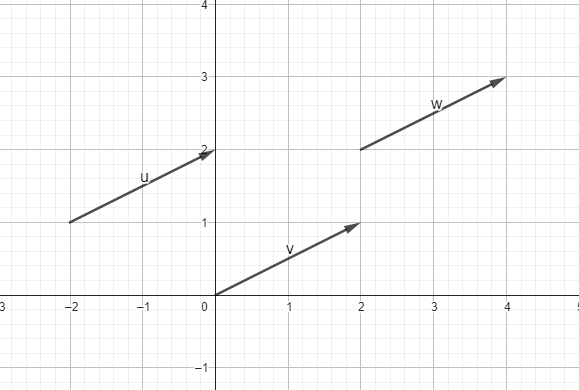
\includegraphics{./images/Vektoren-1-Drei-Vektoren-2022-12-20@16-17-46.png}
        }
    \end{figure}
    Koordinatensystem mit dem Vektor $\vec{v} = \m{2 \\ 1}$ in drei verschiedenen Positionen.

    \subsection{Vektoren 2}
    \begin{figure}[h]
        \centering
        \scalebox{0.5}{
            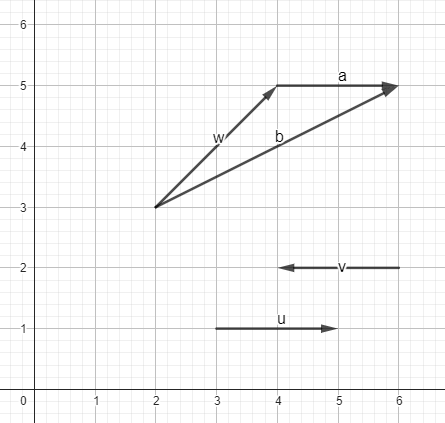
\includegraphics{./images/Vektoren-2-Rechnen-2022-12-19@16-38-25.png}
        }
    \end{figure}
    Multipliziert man den Vektor $\vec{u}$ mit $-1$, erhält man so den Vektor $\vec{v}$.
    Addiert man die Vektoren $\vec{w}$ und $\vec{a}$ resultiert der Vektor $\vec{b}$.

    \newpage

    \subsection{Vektoren 3}
    \begin{figure}[h]
        \centering
        \scalebox{0.5}{
            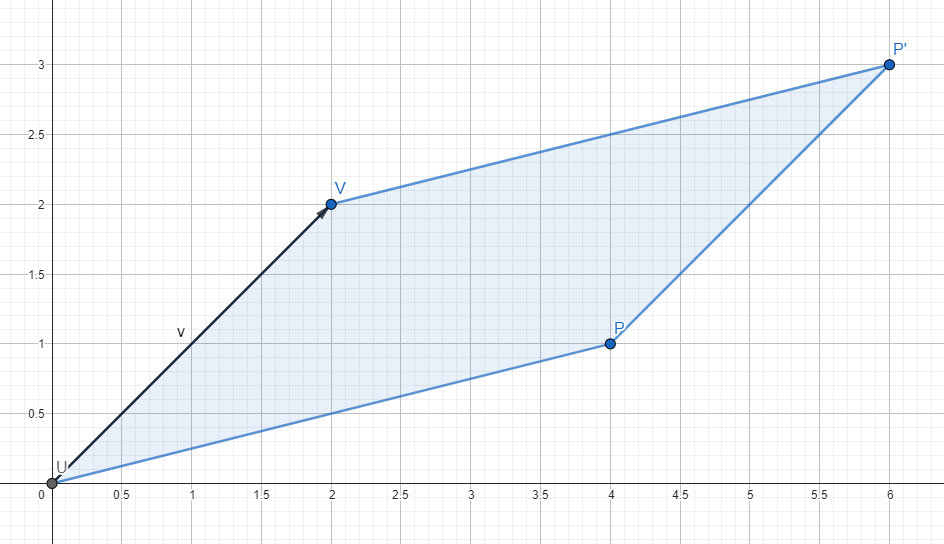
\includegraphics{./images/Vektoren-3-Verschiebung-am-Parallelogramm-2022-12-19@16-30-31.png}
        }
    \end{figure}
    Der Punkt $P$ wird mit dem Vektor $\vec{UV}$ verschoben. Durch das Paralellogramm ergibt sich der neue Punkt $P'$. 
    Der Vektor $\vec{UV}$ ist dabei der Vektor zwischen den beiden Punkten $U$ und $V$ und wird folgendermaßen beschrieben:
    \[
        \vec{v} = \vec{UV} = V - U
    \]

    \subsection{Vektoren 4}
    \begin{figure}[h]
        \centering
        \scalebox{0.5}{
            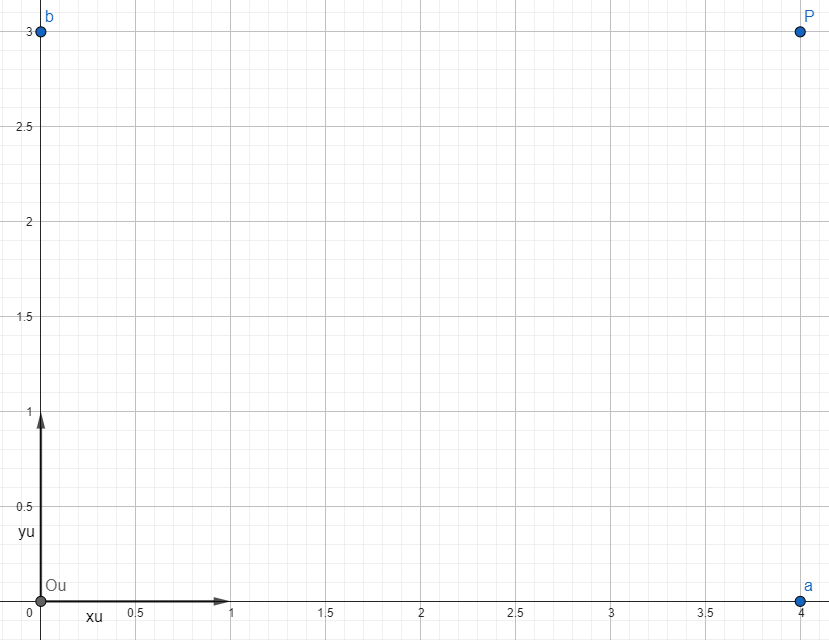
\includegraphics{./images/Vektoren-4-Einheitsvektoren-2022-12-19@17-04-43.png}
        }
    \end{figure}
    Einheitsvektoren $xu$ und $yu$ im Koordinatensystem $U$ mit dem Punkt $P$ und seinen beschreibenden Abschnitten $a$ und $b$.
    
    \newpage


    \subsection{Vektoren 5}
    \begin{figure}[h]
        \centering
        \scalebox{0.5}{
            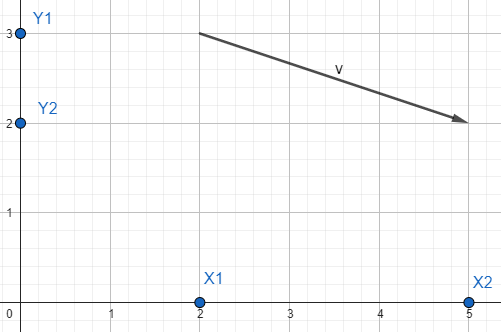
\includegraphics{./images/Vektoren-5-Vektoren-Delta-2022-12-20@16-30-21.png}
        }
    \end{figure}
    Der Vektor $\vec{v}$ wird durch die Differenz des Anfangs- und Endpunktes des Vektors dargestellt.
    \[
        \vec{v} = \m{\Delta{x} \\ \Delta{y}} = \m{X2 - X1 \\ Y2 - Y1} = \m{5 - 2 \\ 2 - 3} = \m{3 \\ -1}
    \]


    \subsection{TITEL}
    \begin{figure}[h]
        \centering
        \scalebox{0.5}{
            
\includegraphics{./images/Mathemann.png}
        }
    \end{figure}

\end{document}


% Notizen und Hilfen

% Der Satz des Pytagoras lautet: $a^2 + b^2 = c^2$.
% Die PQ-Formel latuet:
    
% \[
%     x = - \frac{p}{2} \pm \sqrt{ \left ( \frac{p}{2}^2 \right ) - q }
% \]

% \[
%     \begin{pmatrix}
%         1 & 2 & 3 \\
%         4 & 5 & 6 \\
%         7 & 8 & 9

%     \end{pmatrix}
% \]
